%\part{Konstruktion}
%\chapter{Programmlogik}

\section{SEARCHExtraction}
Die \lstinline|SEARCHExtraction| nimmt ein \lstinline|WebContent|-Objekt entgegen und verarbeitet es zu einem \lstinline|SEARCHModels|-Objekt. Hierbei wird der HTML-Code, der im \lstinline|WebContent| enthalten ist, auf \SEARCH-Tags abgesucht. Diese \SEARCH-Tags werden dann zu einzelnen \lstinline|SEARCHModel|-Objekten zusammengebaut und in einem gemeinsamen \lstinline|SEARCHModels|-Objekt gesammelt.

Für den Ablauf der Analyse und die Erzeugung des \lstinline|SEARCHModels|-Objektes ist der \lstinline|SearchManager| zuständig. Die Methoden für die Analyse des HTML-Codes stellt die \lstinline|RegexForSEARCH| zur Verfügung.

\begin{figure}[h]
	\centering
	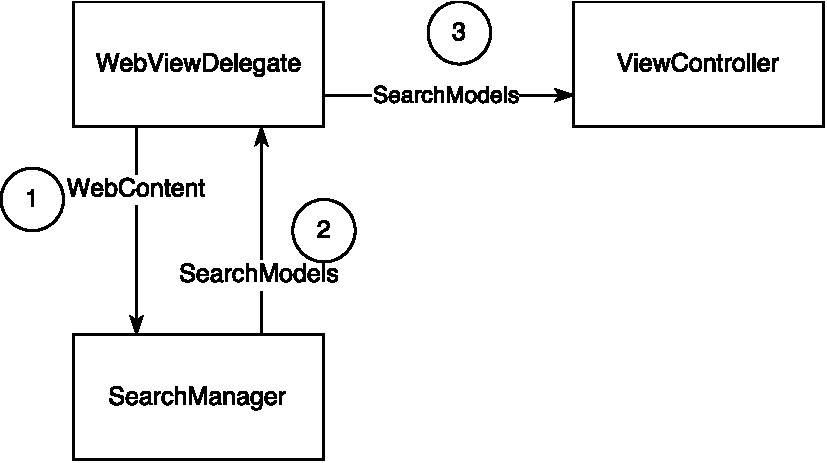
\includegraphics[width=\textwidth]{UI_WebContent_SearchModel_Usage}
	\caption{Umwandeln eines WebContent-Objekts in ein \lstinline|SEARCHModels|-Objekt}
\end{figure}

Die Darstellung beschreibt den Ablauf und die Schnittstellen zwischen dem \lstinline|WebContent| und dem \lstinline|SEARCHModels|-Objekt. Der \lstinline|WebContent|, erzeugt vom \lstinline|WebViewDelegate|, wird in Schritt 1 dem \lstinline|SearchManager| übergeben. Der \lstinline|SearchManager| erzeugt dann aus dem \lstinline|WebContent| das \lstinline|SEARCHModels|-Objekt und gibt dieses im folgenden Schritt 2 an den \lstinline|WebViewDelegate| zurück. Der \lstinline|WebViewDelegate| übergibt nun das \lstinline|SEARCHModels|-Objekt an den \lstinline|ViewController|, wo es schließlich für die anderen Packages zur Verfügung  steht.